\documentclass[UTF8,a4paper,zihao=-4]{ctexart}
\usepackage[margin=2.5cm]{geometry}
\usepackage{graphicx,caption,amsmath,lmodern,float}
\captionsetup{font=small,labelsep=quad}
\pagestyle{empty}
\begin{document}
药材内部的温度与含水率分布具有不同特征。图\ref{fig:mechanism}以问题二的同一时刻为例，把内部径向分布与表面交换方向对应起来：外层温度较高，而中心仍保留较高含水率。两场通过附录3规定的局部物性关系相互影响。

\begin{figure}[H]
\centering
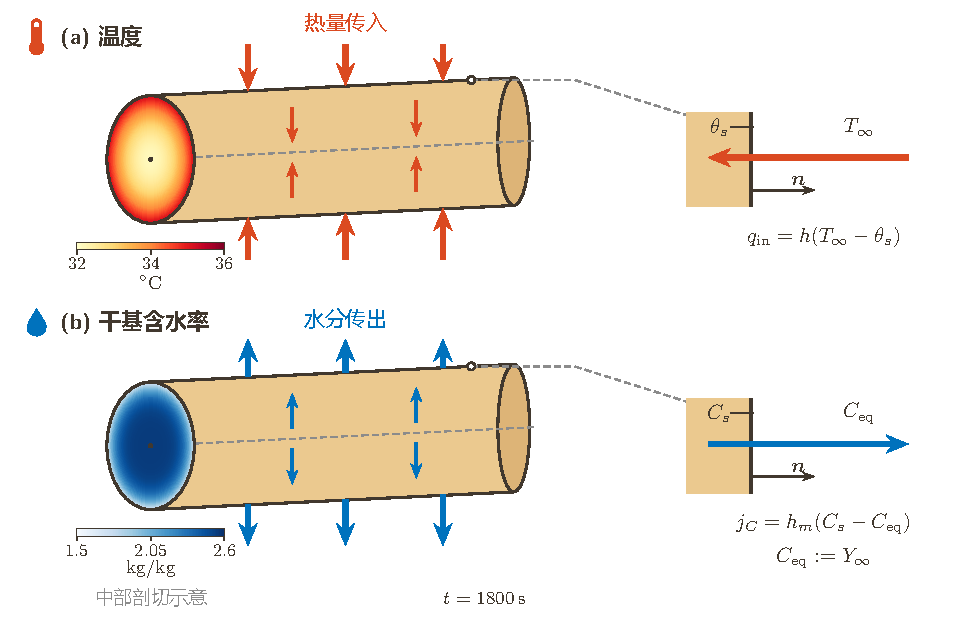
\includegraphics[width=\linewidth]{fig_mechanism_v2.pdf}
\caption{药材中部温湿分布与侧表面传热传质示意}
\label{fig:mechanism}
\smallskip
\begin{minipage}{\linewidth}\small
两行表示同一药材在 $t=1800\,\mathrm{s}$ 时的两个物理量；仅中部切面按问题二未舍入结果着色，色标分别对应温度和干基含水率。圆柱侧体的金黄色用于识别材料，几何与箭头未按数值比例绘制。此时 $T_\infty>\theta_s$、$C_s>C_{\rm eq}$，热量向内、水分向外交换；$q_{\rm in}$ 取向内为正，$j_C$ 表示所选模型的含水率交换通量。$C_{\rm eq}:=Y_\infty$。
\end{minipage}
\end{figure}
\end{document}
